\documentclass[12pt]{article}

% Packages
\usepackage{amsmath}
\usepackage{amsthm}
\usepackage{graphicx}
\usepackage{hyperref}
\usepackage{geometry}
\usepackage{fancyhdr}
\usepackage{cite}
\usepackage{algorithm}
\usepackage{algorithmic}
\usepackage{pgfplots}
\pgfplotsset{compat=1.18}

% Page layout
\geometry{a4paper, margin=1in}
\setlength{\headheight}{14.49998pt}
% Header and Footer
\pagestyle{fancy}
\fancyhf{}
\fancyhead[C]{Survey of Randomized Techniques in Graph Algorithms}
\fancyhead[R]{\thepage}

% Title
\title{Survey of Randomized Techniques in Graph Algorithms}
\author{
    Wang Xianbang\thanks{Email: \texttt{wang-xb24@mails.tsinghua.edu.cn}} \\
    IIIS, Tsinghua University
    \and
    Lu Yiyang\thanks{Email: \texttt{WOBUZHIDAO@mails.tsinghua.edu.cn}} \\
    IIIS, Tsinghua University
}

\newtheorem{lemma}{Lemma}
\newtheorem{theorem}{Theorem}

\begin{document}

\maketitle

% Abstract
\begin{abstract}
    Sheng Si Ju Ji Xue Bing Wang, Jian Xian Si Qi Fu Tou Bang.\\
    \textbf{Abstract:} This is a survey on randomized algorithms on graphs. We focus on two well-known problems: All Pairs Shortest Path (APSP) and Min Cut. We introduce the deterministic algorithms for these problems, and then present the randomized algorithms. We analyze the time complexity and success probability of the randomized algorithms, and provide experimental results. You can find the source code of the algorithms in \url{https://github.com/PeppaKing8/algdesign-project}.\\
    \textbf{Keywords:} Randomized Algorithms, Graph Theory, APSP, Min Cut
\end{abstract}

% Introduction
\section{APSP: All Pairs Shortest Path}
\subsection{Introduction}

One of the well-known result in randomized algorithms in graph theory is the algorithm for the \textbf{All Pairs Shortest Path (APSP)} problem.

Let $G(V,E)$ be an \textbf{undirected} graph, with $V=\{1,2,\cdots,n\}$ and $|E|=m$. Let the adjacency matrix of $G$ be $A$, where $A_{ij}=A_{ji}=1$ if $(i,j)\in E$ and $A_{ij}=A_{ji}=0$ otherwise. There is a weak version of the APSP problem, \textbf{All Pairs Distance (APD)} problem, which is to compute the distance between all pairs of vertices in $G$, i.e., derive the \emph{distance matrix} $D$ where $D_{ij}$ is the length of the shortest path between $i$ and $j$.

The requirement of APSP is stronger: it requires the algorithm to compute the shortest path itself, not just the length of the shortest path, of all pairs of vertices in $G$. 

If $G$ is not connected, we can seperate $G$ into connected components and solve the APSP problem for each connected component (finding connected components is easy and can be done in linear time). So we assume $G$ is \textbf{connected} in the following discussion.

Note that, if we want to store all the shortest paths, the space complexity can be $\Omega(n^3)$ (e.g. a path), which limits the time complexity we can achieve. However, we can record an \emph{implicit} representation of the shortest path - the \textbf{successor matrix} $S$: for every $(u,v)\in V^2$, let $S_{uv}$ be the vertex that is the immediate successor of $u$ on the shortest path from $u$ to $v$. This can be stored in $O(n^2)$ space, and the shortest path from $u$ to $v$ can be reconstructed by following the path $u\to S_{uv}\to S_{S_{uv}v}\to\cdots\to v$ in $O(L)$ time, where $L$ is the length of the shortest path.

\subsection{Quick Review on Deterministic Algorithms}

The most well-known algorithm for APSP is the \textbf{Floyd-Warshall} algorithm, which has a time complexity of $O(n^3)$. The algorithm is based on dynamic programming, and the key idea is to consider all vertices as potential intermediate vertices in the shortest path. The algorithm is simple and easy to implement.

Another algorithm is based on \textbf{breadth-first search (BFS)}: for every vertex $v$, run a BFS starting from $v$ to compute the shortest path from $v$ to all other vertices. This algorithm has a time complexity of $O(nm)$, which is better when $m=o(n^2)$.

For weighted graph (every edge has a weight), the \textbf{Johnson} algorithm can be used to solve the APSP problem. The time complexity can achieve $O(nm+n^2\log n)$ using Fibonacci heap. This algorithm is an extension of Dijkstra's algorithm, which is only applicable in non-negative weight circumstance. 

It is clear that the best time complexity we can achieve for APSP is $\Omega(n^2)$, since we need to output $n^2$ shortest paths. And we also believe that $O(nm)$ is still far away from the best, especially if $m=\Omega(n^2)$.

\subsection{Matrix Multiplication-based Algorithm}

Now we introduce a randomized algorithm for APSP, which is based on matrix multiplication. The algorithm is proposed by Alon, Galil, and Margalit in 1994.

\subsubsection{Skim on Matrix Multiplication}

Given two $n\times n$ matrices $A$ and $B$, the product $C=AB$ is defined as $C_{ij}=\sum_{k=1}^n A_{ik}B_{kj}$. The naive algorithm has a time complexity of $O(n^3)$. The lower bound of matrix multiplication is obviously $\Omega(n^2)$, and computer scientists have been trying to find a better exponent $2<\alpha<3$ until now.

Strassen proposed a divide-and-conquer algorithm in 1969, which has a time complexity of $O(n^{\log_2 7})\approx O(n^{2.81})$. According to Wikipedia, as of January 2024, the best peer-reviewed matrix multiplication algorithm is by Virginia Vassilevska Williams, Yinzhan Xu, Zixuan Xu, and Renfei Zhou and has complexity $O(n^{2.371552})$. It is still an open problem to find a matrix multiplication algorithm with complexity $O(n^{2+o(1)})$, or prove that such an algorithm does not exist.

\emph{From now on, suppose we have a matrix multiplication algorithm with time complexity $O(n^\nu)$.}

\subsubsection{APD}
Recall that $A$ is adjacent matrix. Let $\bar{A}$ be the matrix where $\bar{A}_{ij}=1$ if $i=j$ or $A_{ij}=1$. The connection between shortest path and matrix multiplication is revealed by the following lemma.
\begin{lemma}
    \label{lemma:shortest_path_matrix_multiplication}
    Let $k$ be an positive integer. For every $i,j\in V$, $D_{ij}\le k$ if and only if $\bar{A}^k_{ij}>0$.
\end{lemma}
\begin{proof}
If $\bar{A}^k_{ij}>0$, considering the procedure of matrix multiplication, there must be $i_0=i,i_1,i_2,\cdots,i_k=j\in V$, such that $\bar A_{i_0i_1}=\bar A_{i_1i_2}=\cdots=\bar A_{i_{k-1}i_k}=1$. So there is a path $i_0\to i_1\to i_2\to\cdots\to i_k$ of length $k$ from $i$ to $j$, which implies $D_{ij}\le k$.
\end{proof}

The lemma implies that we can compute the distance matrix $D$ by computing $\bar{A}^k$ for $k=1,2,\cdots,n$. However, this requires $O(n^{\nu+1})=\omega(n^3)$ time, which is even worse.

The idea to improve this is: we compute $\bar A^2$, which can reduce the length of the shortest path to a half, and do the computation recursively. We should first get $A'$, where $A'_{ij}=1$ if $A_{ij}=1$ or there is a path of length 2 from $i$ to $j$. From Lemma \ref{lemma:shortest_path_matrix_multiplication}, we can derive $A'$ from $\bar A^2$ in $O(n^2)$: $A'_{ij}=1$ iff $\bar A_{ij}>0$.

Recursively run the algorithm on $A'$ (which also represents a graph $G'$), and suppose we got a distance matrix $D'$ for $G'$. Now we want to retrieve $D$.

\begin{lemma}
\label{2}
For every $i,j\in V$, $D'_{ij}=\lceil\dfrac{D_{ij}}{2}\rceil$.
\end{lemma}
\begin{proof}
Due to the definition of $A'$, $D'$ represents the distance, where we can walk 2 steps at a time. The lemma is then obvious.
\end{proof}

Lemma \ref{2} is inadequate because given $D'$, every element of $D$ has two choices. However, Lemma \ref{3} could tell us the answer.
\begin{lemma}
\label{3}
Let $i\not=j \in V$. For any neighbor $u$ of $i$ in $G'$, $D_{ij}-1\le D_{uj}\le D_{ij}+1$. And there exists at least one $u$, such that $D_{uj}=D_{ij}-1$.
\end{lemma}
\begin{proof}
For any neighbor $u$, we can first go to $i$, and walk $D_{ij}$ steps to $j$. Thus, there is a path from $u$ to $j$ of length $D_{ij}+1$, implying $D_{uj}\le D_{ij}+1$. Interchange $i$ and $u$, we can get $D_{uj}\ge D_{ij}-1$. Suppose the shortest path between $i,j$ is $i\to i_1\to\cdots\to i_t=j$, then $D_{i_1j}=D_{ij}-1$.
\end{proof}

\begin{lemma}
\label{4}
If $D_{ij}$ is even, $D'_{kj}\ge D'_{ij}$ for every neighbor $k$ of $i$; if $D_{ij}$ is odd, $D'_{kj}\le D'_{ij}$ for every neighbor $k$ of $i$, and at least one equality does not hold.
\end{lemma}
\begin{proof}
Suppose $D_{ij}=2t$ is even. Lemma \ref{3} tells $D_{kj}\in\{2t-1,2t,2t+1\}$ for every neighbor $k$ of $i$. Use Lemma \ref{2}, $D'_{kj}\ge t=D'_{ij}$. \\
Now suppose $D_{ij}=2t+1$ is odd, then $D_{kj}=\{2t,2t+1,2t+2\}$, so $D'_{kj}\in \{t,t+1\}$, thereby $\le t+1=D'_{ij}$. And at least one $k$ satisfies $D_{kj}=D_{ij}-1=2t$, so $D'_{kj}=t<D'_{ij}$.
\end{proof}

In fact, to compute $D$ from $D'$, we only need to know the parity of each $D_{ij}$. From Lemma \ref{4}, we can seperate even and odd $D_{ij}$, and compute $D$ in $O(n^2)$ time. Specifically, $D_{ij}$ is even iff
$$\sum\limits_{k\text{ is neighbor of }i} D'_{kj}\ge d_iD_{ij},$$
$d_i$ is the degree of $i$. If $S=AD'$, then $D_{ij}$ is even iff $S_{ij}\ge d_iD_{ij}=\bar A^2_{ii}D_{ij}$. The implementation is shown in Algorithm \ref{alg:example}.

\begin{algorithm}
\caption{APD}
\label{alg:example}
\begin{algorithmic}
    \STATE \textbf{Input:} Graph $G=(V,E)$ with adjacency matrix $A$
    \STATE \textbf{Output:} Distance matrix $D$
    \STATE $\bar A\leftarrow I+A$
    \STATE $A^*\leftarrow \bar A^2$
    \FOR{$i=1$ to $n$}
        \FOR{$j=1$ to $n$}
            \STATE $A'_{ij}\leftarrow 1$ if $A_{ij}=1$ or ${A^*}_{ij}>0$
        \ENDFOR
    \ENDFOR
    \STATE $D'\leftarrow$ APD$(A')$
    \STATE $S\leftarrow AD'$
    \FOR{$i=1$ to $n$}
        \FOR{$j=1$ to $n$}
            \STATE $D_{ij}\leftarrow 2D'_{ij}$ if $S_{ij}\ge A^*_{ii}D'_{ij}$, otherwise $D_{ij}\leftarrow 2D'_{ij}-1$
        \ENDFOR
    \ENDFOR
    \RETURN $D$
\end{algorithmic}
\end{algorithm}

\subsubsection{APSP}

Observe that, the preceding algorithm does not provide enough information of successor matrix $S$. More precisely, if $D_{ij}$ is even, it is not guaranteed from Lemma \ref{4} that we can find $k$ just from $D'$.

Suppose $D$ is computed with algorithm \ref{alg:example}. For every $i,j\in V$, how to find $S_{ij}$? Or, what is the necessary and sufficient condition of $S_{ij}$? The answer of the last question is clear: $(i,S_{ij})\in E$, and $D_{ij}-1 = D_{S_{ij}j}$. Let $r=D_{ij}$. For every integer $u\ge 0$, define $D^{(u)}$ as: $D^{(u)}_{ij}=1$ iff $D_{ij}=u$. So $S_{ij}$ is one of the \textbf{witness} of $A$ and $D^{(r-1)}$ w.r.t $i,j$. (\emph{Note: the witness of two matrices $A$ and $B$ w.r.t. $i,j$ is an index $x$ that $A_{ix}=B_{xj}=1$.})

Given two 0-1 matrices $A,B$, to compute a \textbf{witness matrix} is a well-known problem in computer science called \textbf{Boolean Product Witness Matrix (BPWM)}. We will leave the implementation of BPWM in section \ref{sec:bpwm}. Now assume we have a black box \texttt{BPWM(A,B)}.

From the above discussion, we need to enumerate $r=1,2,\cdots,n$ and compute $D^{(r-1)}$ for each $r$, and derive the witness matrix of $A$ and $D^{(r-1)}$, which needs $O(n)$ times of \texttt{BPWM}. However, a clever optimization can reduce to only $3$ times. For $s=0,1,2$, Let $D^{[s]}$ be the matrix where $D^{[s]}_{ij}=1$ iff $D_{ij}\equiv s\pmod 3$. Denote the witness of $A$ and $D^{[s]}$ by $W^{[s]}$.

\begin{lemma}
\label{5}
For every $i,j\in V$, $S_{ij}=W^{[(D_{ij}-1)\mod 3]}_{ij}$.
\end{lemma}
\begin{proof}
Firstly, $S_{ij}$ is a witness of $A$ and $W^{[(D_{ij}-1)\mod 3]}$. This is because $(i,S_{ij})\in E$, and $D_{S_{ij}j}=D_{ij}-1$, thereby also $\equiv D_{ij}-1\pmod 3$. Note that this also implies that $W^{[(D_{ij}-1)\mod 3]}_{ij}$ exists.\\
On the other hand, suppose $v=W^{[(D_{ij}-1)\mod 3]}_{ij}$. Then $D_{vj}\equiv D_{ij}-1\pmod 3$, and $v$ is a neighbor of $i$. Since from Lemma \ref{3}, $D_{vj}\in [D_{ij}-1,D_{ij}+1]$, we immediately get $D_{vj}=D_{ij}-1$, which means $v$ is one of the successor.
\end{proof}

Thus, if $W^{[s]}(s=0,1,2)$ is computed, $S$ can be derived in $O(n^2)$ time. The time complexity is $O(f(n)+n^2)$, where $f(n)$ is the time complexity of \texttt{BPWM}, obviously $\Omega(n^2)$.

\subsubsection{BPWM}
\label{sec:bpwm}

Recall that the input of BPWM is two 0-1 $n\times n$ matrices $A,B$, and the output is a matrix $W$, where $W_{ij}$ is the witness of $A$ and $B$ w.r.t. $i,j$.

Consider a simple case: assume for every $i,j$, the witness is \textbf{unique}. Define a``weighted'' matrix $A^{\#}$ as: $A^{\#}_{ik}=kA_{ik}$. Now, we compute $W^{\#}=A^{\#}B$. Since $A^{\#}$ is weighted - intuitively, the vertex $i$ has value $i$. From the definition of $W^{\#}$, $W^{\#}_{ij}$ is the sum of the values of all the witnesses. Since the witness is unique, $W^{\#}_{ij}$ is the value of the witness. So we can derive $W$ from $W^{\#}$ in $O(n^2)$ time - $W=W^{\#}$, actually.

Now consider the general case. We continue to use the ``weighted'' idea, but just choose a \textbf{subset} of $V$ to be the weighted. If we are lucky, the witness is unique within the subset, and we are done. We will see that randomization give us that luck.

For every $i,j$, suppose there are $t$ witnesses. From easy math, there exists a positive integer $r$, such that $\dfrac{n}{2}\le tr\le n$. Randomly choose a subset of rank $r$ of $V$, and weight them with their own index. For other $n-r$ vertices, weight them with $0$. The following lemma shows the probability of choosing a unique witness is larger than a positive constant!

\begin{lemma}
\label{6}
Let $v=\{1,2,\cdots,n\}$, $S_0=\{1,\cdots,t\}$, integer $r$ satisfies $\dfrac{n}{2}\le tr\le n$. Randomly choose a subset $S\subseteq V$ of rank $r$. We have
$$P(|S\cap S_0|=1)\ge \dfrac{1}{2e}.$$
\end{lemma}
\begin{proof}
Since $tr\le n$, we have $\dfrac{r-1}{n-t}\le \dfrac{1}{t}$. The probability is
\begin{align*}
\dfrac{t\cdot \binom{n-t}{r-1}}{\binom{n}{r}} &= t\cdot \dfrac{(n-t)!r!(n-r)!}{(r-1)!(n-t-r+1)!n!}\\
&= \dfrac{tr}{n}\cdot \dfrac{(n-t)!(n-r)!}{(n-t-r+1)!(n-1)!}\\
&= \dfrac{tr}{n}\cdot \prod\limits_{i=0}^{t-2} \dfrac{n-r-i}{n-1-i}\\
&\ge \dfrac{tr}{n}\cdot \left(1-\dfrac{r-1}{n-t}\right)^{t-1}\\
&\ge \dfrac{1}{2}\cdot \left(1-\dfrac{1}{t}\right)^{t-1} \ge \dfrac{1}{2e}.
\end{align*}
\end{proof}

Lemma \ref{6} shows that, if we try $L$ different subsets, the probability to fail (i.e. in each case $|S\cup S_0|\not=1$) will be $O(\exp{\Theta(n)})$. Lemma \ref{7} shows that we can choose appropiate $r$ within a set of $O(\log n)$ candidates.

\begin{lemma}
\label{7}
For every $1\le t\le n$, there exists a natural number $k\le \log n$, such that $\dfrac{n}{2}\le t\cdot 2^k\le n$.
\end{lemma}
\begin{proof}
Let $k$ be the largest integer such that $t\cdot 2^k\le n$. Then $t\cdot 2^{k+1}>n$, so $t\cdot 2^k\le n/2$. And $2^k\le t\cdot 2^k\le n$, so $k\le \log n$, as desired.
\end{proof}

So the algorithm is as follows: enumerate every $r=1,2,\cdots,2^{\lfloor\log n\rfloor}$. For every $r$, randomly choose $L=\Theta(\log n)$ subsets of rank $r$, and compute the witness matrix. For every $i,j$, Lemma \ref{6} tells us the probability to fail is $o(\dfrac{1}{n^2})$ if $\lim\limits_{n\to \infty}\dfrac{L}{\log n}$ is sufficiently large. Then the union bound directly bounds the failing probability by $o(1)$.

If we have missed some witness (which is very unlucky), we found these missing witnesses by brute-force - $O(n)$ for every pair $(i,j)$. Since the expected number of missing pair is $O(1)$, the time complexity of this procedure can be ignored.

In practice, we set $L=\gamma\log n$, where $\gamma$ is a constant. We pick $\gamma=3$ in practice, considering the trade-off between time complexity and success probability. 

The whole algorithm (APSP) is shown in Algorithm \ref{alg:BPWM}. The black box \texttt{BPWM} is implemented in Algorithm \ref{alg:bp}.

\begin{algorithm}
    \caption{APSP}
    \label{alg:BPWM}
    \begin{algorithmic}
        \STATE \textbf{Input:} Graph $G=(V,E)$ with adjacency matrix $A$
        \STATE \textbf{Output:} Successor matrix $S$
        \STATE $D\leftarrow \text{APD}(A)$
        \FOR{$s\in \{0,1,2\}$}
            \STATE compute $D^{[s]}$ by: $D^{[s]}_{ij}=1$ iff $D_{ij}\equiv s\pmod 3$
            \STATE $W^{[s]}\leftarrow \text{BPWM}(A,D^{[s]})$
        \ENDFOR
        \FOR{$i=1$ to $n$}
            \FOR{$j=1$ to $n$}
                \STATE $r\leftarrow (D_{ij}-1)\mod 3$
                \STATE $S_{ij}\leftarrow W^{[r]}_{ij}$
            \ENDFOR
        \ENDFOR
    \RETURN $S$
    \end{algorithmic}
\end{algorithm}

\begin{algorithm}
    \caption{BPWM}
    \label{alg:bp}
    \begin{algorithmic}
        \STATE \textbf{Input:} 0-1 matrices $A,B$ of size $n\times n$
        \STATE \textbf{Output:} Witness matrix $W$
        \FOR{$t=0,1,\cdots,[\log n]$}
            \STATE $r\leftarrow 2^t$
            \FOR{$l=1$ to $\gamma\log n$}
                \STATE Randomly choose a subset $S$ of rank $r$
                \STATE construct $A^{\#}$: $A^{\#}_{ik}\leftarrow kA_{ik}$ for $i\in S$, $0$ otherwise
                \STATE $W^{\#}\leftarrow A^{\#}B$
                \FORALL{$(i,j)$}
                    \STATE $W_{ij}\leftarrow W^{\#}_{ij}$ if $W_{ij}$ is not defined and $W^{\#}_{ij}$ is a witness
                \ENDFOR
            \ENDFOR
        \ENDFOR
        \FORALL{$(i,j)$}
            \IF{$W_{ij}$ is not defined}
                \STATE $W_{ij}\leftarrow$ brute-force to find the witness
            \ENDIF
        \ENDFOR
    \RETURN $W$
    \end{algorithmic}
\end{algorithm}

\subsubsection{Time Complexity Analysis}

\paragraph{APD} APD is a deterministic algorithm and it performs recursively. Since every recursion we reduce the length of the shortest path by a half, the depth of the recursion is $O(\log n)$. In every recursion, we need to compute $A^*$ and $S$, which takes $O(n^{\nu})$ time (recall that this is the hypothesized time complexity of matrix multiplication). Other procedures just take $O(n^2)=o(n^{\nu})$ time. So the time complexity of APD is $O(n^{\nu}\log n)$.

\paragraph{BPWM} Consider $(t,l)$, we have $O(\log n\cdot \log n)=O(\log^2 n)$ pairs. For every pair, we need to compute $W^{\#}$, which takes $O(n^{\nu})$ time. Other procedures take $O(n^2)$ time. So the time complexity of BPWM is $O(n^{\nu}\log^2 n)$.

\paragraph{APSP} APSP calls APD and BPWM for constant times, so the time complexity is $O(n^{\nu}\log^2 n)$.

\subsubsection{Small Improvement}
\label{imp}

Use carefully analysis, we can actually show that BPWM is $O(n^\nu \log n)$, so APSP is also $O(n^\nu \log n)$. The key idea is, $A^\#$ can be reduced to $n\times r$, so $W^\#$ is actually multiplication of two matrices of size $n\times r$ and $r\times n$ respectively.

For matrix of size $n\times r$, divide it into $\lfloor\dfrac{n}{r}\rfloor$ blocks (by row). For $r\times n$ matrix is similar. Then we can compute each pair of blocks in $O(r^{\nu})$ time, and combine them into one single $n\times n$ matrix in $O(n^2)$ time. So the time complexity of this multiplication is $O(r^\nu(\dfrac{n}{r})^2)=O(r^{\nu-2}n^2)$.

So, the time complexity of BPWM is
\begin{align*}
\sum\limits_{t=0}^{\log n}\sum\limits_{l=1}^{\gamma\log n} O(r^{\nu-2}n^2) &= \gamma\log n\cdot \sum\limits_{t=0}^{\log n} O(r^{\nu-2}n^2)\\
&= \gamma\log n\cdot O(n^2)\cdot \sum\limits_{t=0}^{\log n} O(2^{t(\nu-2)})\\
&= \gamma\log n\cdot O(n^2)\cdot O(n^{\nu-2}) = O(n^\nu\log n)
\end{align*}
if $\nu>2$.

\subsection{Experimental Results}

We implemented four algorithms for APSP: for the deterministic algorithms, we implemented Floyd-Warshall and BFS; for the randomized algorithms, we implemented the matrix multiplication-based algorithm with two versions: one with Strassen's algorithm and the other with the trivial matrix multiplication. The latter two is the improved version of the algorithm in section \ref{imp}.

Algorithms are implemented with C++.

\subsubsection{Settings}

We set the graph size to be $n=2^k$, where $k\le 8$. In our experiment, edges are independently and uniformly generated, each with probability $p$. To ensure the graph is connected, after graph is randomly generated, we add $M-1$ edges to connect the graph, where $M$ is the number of connected components.

Our test environment is $\texttt{-std=C++11}$ and has unlimited stack size. 

\subsubsection{Parameters}

We set $\gamma=3$ in BPWM, and the threshold of Strassen's algorithm to be $n_0=64$. $p=0.1$ since we do not want the graph to be too dense, and also limit the performance of BFS.

\subsubsection{Results}

We run the algorithms for 5 times and record the average execution time. The results of $k=7,8$ ($n=128,256$) are shown in Figure \ref{fig:et}. 

An interesting phenomenon is, when $k$ increase by 1, the execution time of \texttt{BFS} and \texttt{Floyd} increase by a factor of $3\sim 4$, while the execution time of \texttt{Strassen} and \texttt{Trivial} increase by a factor of $5\sim 6$. This is partially due to the optimization of C++ compiler, which can optimize the loops in \texttt{BFS} and \texttt{Floyd} to be more cache-friendly - but not the case when there are heavy matrix multiplications.

\begin{figure}[h]
    \centering
    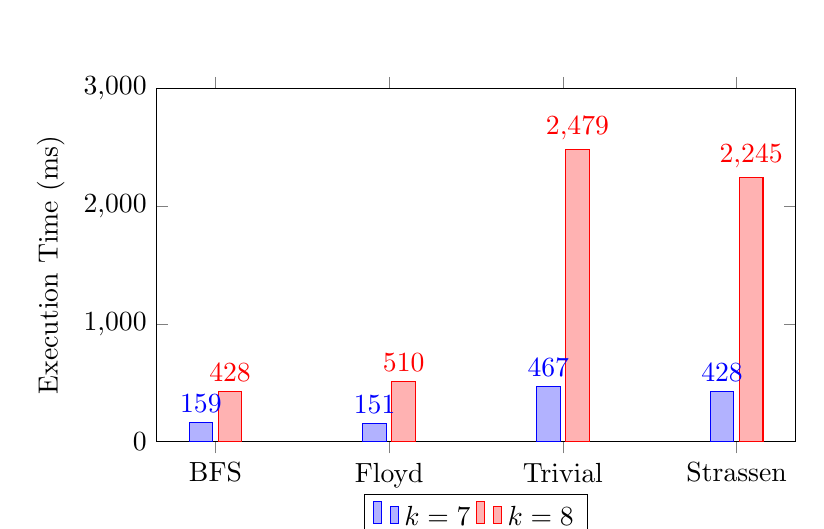
\begin{tikzpicture}
        \begin{axis}[
            ybar,
            bar width=0.3cm,
            width=0.8\textwidth,
            height=0.5\textwidth,
            symbolic x coords={BFS, Floyd, Trivial, Strassen},
            xtick=data,
            ylabel={Execution Time (ms)},
            xlabel={Algorithms},
            ymin=0,
            ymax=3000,
            legend style={at={(0.5,-0.15)}, anchor=north, legend columns=-1},
            nodes near coords,
            enlarge x limits={abs=0.75cm}
        ]
        \addplot coordinates {(BFS, 159) (Floyd, 151) (Trivial, 467) (Strassen, 428)};
        \addplot coordinates {(BFS, 428) (Floyd, 510) (Trivial, 2479) (Strassen, 2245)};
        \legend{$k=7$, $k=8$}
        \end{axis}
    \end{tikzpicture}
    \caption{Execution time of different algorithms on two datasets}
    \label{fig:et}
\end{figure}

\subsubsection{Analysis}

Granted, although the time complexity of \texttt{Strassen} is better than \texttt{BFS} and \texttt{Floyd}, the actual execution time is much larger. This is because the constant factor of Strassen's algorithm is remarkably large. Moreover, if the parameter is not carefully chosen, or $p$ is much smaller, \texttt{BFS} will perform even better and \texttt{Strassen} and \texttt{Trivial} will be even worse. Consequently, the matrix multiplication-based algorithm has less practical significance than theoretical significance.

Based on the data of $k=8$, we can approximate the constant factor of these algorithms. Suppose the execution time of \texttt{Floyd} is $\beta\cdot n^3$, and the execution time of \texttt{Strassen} is $\alpha\cdot n^{\log_2 7}\log n$. Plugging in the data, we can get $\alpha\approx 3.9\cdot 10^{-4}$ and $\beta\approx 8.5\cdot 10^{-5}$. Finding the threshold $N$, which satisfies $\alpha\cdot N^{\log_2 7}\log N=\beta\cdot N^3$, we can get $N\approx 2500$. 

Since for $n=2^k$, Strassen's algorithm is much faster than other cases (which need to expand the matrix up to $4$ times of parameters), we can extrapolate that the actual threshold should be $N_0\approx 10^4$. \texttt{Strassen} will likely be faster than \texttt{Floyd} when $n\gg N_0$; if we replace Strassen's matrix multiplication with the most advanced algorithm, we surmise that the threshold will be slightly lower.

\subsection{Extensions}

\subsubsection{Derandomization}
\subsubsection{Directed Graph}
\subsubsection{Weighted Graph}

\subsection{Open Problems}
\section{Min Cut}

\subsection{Introduction}
\textbf{Min Cut} problem is a well-known problem in graph theory. The problem is defined as follows: given a  undirected graph $G(V,E)$, with $V=\{1,2,\cdots,n\}$ and $|E|=m$, define the adjacent matrix $A$, where $A_{ij}=A_{ji}=1$ if $(i,j)\in E$ and $A_{ij}=A_{ji}=0$ otherwise. A \textbf{cut} of $G$ is a partition of $V$ into two sets $S$ and $V\backslash S$, where $S\neq\emptyset$ and $V\backslash S\neq\emptyset$. The \textbf{cost} of a cut $(S,V\backslash S)$ is defined as
\begin{align*}
    \text{cost}(S,V\backslash S)=\sum_{i\in S, j\in V\backslash S}A_{ij}
\end{align*}

The Min Cut problem is to find a cut $(S,V\backslash S)$ with the minimum cost.
\subsection{Quick Review on Deterministic Algorithms}
Deterministic algorithms for minimum cut problem are initially derived from minimum $s-t$ cut problem, which aims to find a partition that separates $s$ and $t$ and minimizes the weight between the edges. It's well known that 
\begin{lemma}
    In a undirected graph $G(V,E)$, given two vertices $s,t\in V$, the minimum $s-t$ cut equals the maximum $s-t$ flow.
\end{lemma}
To find the global minimum cut, a naive thought is exexuting maximum flow algorithm for $s=0,t=1,\cdots,n-1$, which has a time complexity of $O(n\text{MF}(n,m))$, where $\text{MF}(n,m)$ is the time complexity of maximum flow algorithm. Since the best deterministic maximum flow problem runs in time $O(mn\log(n^2/m))$, using this naive approach would requires $\Omega(n^2m)$. 

Fortunately, using \textbf{Stoer-Wagner}\cite{stoer1997simple} algorithm, the $n-1$ maximum flow computations can be implemented in the time proportional to the cost of a single maximum flow, which has a time complexity of $O(nm+n^2\log n)$. 

Using a more sophisticated algorithm, we can achieve a lower time complexity. In 2024, the \textbf{SOTA}\cite{doi:10.1137/1.9781611977912.111} of deterministic algorithm of Min Cut runs in $\tilde{O}(n^2)$ time, which is near optimal (since the input size is $\Omega(n+m)$, which is $\Omega(n^2)$ in the worst case).

\subsection{Karger-Stein Algorithm}
Now we introduce a randomized algorithm for Min Cut, which is based on Karger's algorithm\cite{karger1996new}. The algorithm is proposed by Karger and Stein in 1996.

The randomized algorithm of Min Cut is a \textbf{Monte Carlo} algorithm, which runs in $O(cn^2\log^2 n)$ time with a failure probability of $O(1/n^c)$, where $c$ is any constant. The algorithm is based on the following procedure:
\subsubsection{Contract}
\begin{algorithm}
\caption{Contract}
\label{alg:contract}
\begin{algorithmic}
    \STATE \textbf{Input:} A multi-graph $G(V,E)$, a number $k$
    \STATE \textbf{Output:} A graph $G'(V',E')$
    \STATE $G'\leftarrow G$
    \WHILE{$|V'|>k$}
    \STATE choose an edge $(u,v)$ uniformly at random from $E'$
    \STATE merge $u$ and $v$ into a new vertex $w$
    \STATE remove all self-loops
    \ENDWHILE
    \RETURN $G'$
\end{algorithmic}
\end{algorithm}
The multiplicity of an edge is the number of edges between two vertices, it can be represented by an integer weight on the edge. Hence the number of edges in the graph is $O(n^2)$. Each contraction step takes $O(n)$ time, so we get the following lemma:

\begin{lemma}
    For any $n$-vertex multi-graph $G$, the Algorithm \ref{alg:contract} runs in $O(n(n-k))$ time.
\end{lemma}

If we set $k=2$, the algorithm will return a graph with only two vertices, which equals to a cut of original graph. Based on the fact, we claim that

\begin{lemma}
    \label{lemma:cut}
    A cut $C$ is produced by Algorithm \ref{alg:contract} if and only if none of the edges in $C$ is contracted.
\end{lemma}

Intuitively, since the edge $(u,v)$ is chosen uniformly at random, the probability of choosing an edge in $C$ increases as the number of edges in $C$ increases. Hence the min cut is produced with a higher probability than all the other cut. To determine the specific probability, we need to make use of the following fact:

\begin{lemma}
    \label{lemma:degree}
    In an $n$-vertex multi-graph $G$ with min-cut value $k$, no vertex has degree smaller than $k$. The total number of edges $m$ is at least $nk/2$.
\end{lemma}

\begin{lemma}
    \label{lemma:contract}
    Given an edge $(u,v)$, the min-cut value of graph $G/(u,v)$ is at least the min-cut value of $G$.
\end{lemma}

Based on the above lemmas, we can prove the following theorem:

\begin{theorem}
    \label{theorem:contract}
    Suppose that the Algorithm \ref{alg:contract} terminated when there are $k$ vertices left. Then any specific min-cut $K$ survives in the final graph with probability at least $\Omega(k^2/n^2)$.
\end{theorem}
\begin{proof}
    The number of vertices in graph $G'$ decreases by exactly one during each iteration of Algorithm \ref{alg:contract}, at $i$-th iteration, there are $n_i=n-i+1$ vertices. Suppose none of the edges is contracted during the first $i-1$ iterations, accroding to Lemma \ref{lemma:cut} and \ref{lemma:degree}, $K$ is also min-cut of $G'$ annd the number of edges in $G'$ is at least $n_iK/2$. The probability of choosing an edge in $K$ is at most $2/n_i$. It follows that the probability of no edge of $K$ is contracted during Algorithm \ref{alg:contract} is
\begin{align*}
    \Pr[\text{no edge of }K\text{ is contracted}]&\ge\prod_{i=1}^{n-k+1}\left(1-\frac{2}{n-i+1}\right)\\
    &=\prod_{j=k}^n\left(1-\frac{2}{j}\right)=\frac{(k-2)(k-1)}{n(n-1)}=\Omega\left(\frac{k^2}{n^2}\right)
\end{align*}
\end{proof}


If we set $k=2$, the final output is a cut, and the probability of success is $\Omega(1/n^2)$. Repeating the algorithm for $O(n^2\log n)$ times gives a reasonable probability of success. This gives a Monte Carlo algorithm with a time complexity of $O(n^4\log n)$.

\subsubsection{Fast Cut}
The basic problem with Algorithm \ref{alg:contract} with $k=2$ is the success probability, since at the end of the contraction process there is non-negligible probability that an edge of $K$ gets contracted. This suggests us to contract the edges not too much at a time, based on this idea, we can design a new algorithm:

\begin{algorithm}
\caption{Fast Cut}
\label{alg:fastcut}
\begin{algorithmic}
    \STATE \textbf{Input:} A multi-graph $G(V,E)$
    \STATE \textbf{Output:} A cut $(S,V\backslash S)$
    \STATE $n\leftarrow |V|$
    \IF{$n\leq 6$} 
    \STATE compute the min-cut by brute force
    \RETURN min-cut $(S,V\backslash S)$
    \ELSE
    \STATE $t\leftarrow \lceil 1+n/\sqrt{2}\rceil$
    \STATE Using Algorithm \ref{alg:contract}, perform 2 independent contraction processes to obtain graphs $H_1,H_2$ each with $t$ vertices
    \STATE Recursively run Fast Cut on $H_1$ and $H_2$ to get cuts $(S_1,V_1\backslash S_1)$ and $(S_2,V_2\backslash S_2)$
    \RETURN the cut with the smaller cost
    \ENDIF
    % \ELSE $k\leftarrow $
\end{algorithmic}
\end{algorithm}

The algorithm is a recursive algorithm, Algorithm \ref{alg:contract} uses $O(n^2)$ time to reduce the number of vertices to $t$. We obtain the following recurrence for the running time $T(n)$ of Algorithm \ref{alg:fastcut}:
\begin{align*}
    T(n)=2T\left(\lceil 1+\frac{n}{\sqrt{2}}\rceil\right)+O(n^2)
\end{align*}

The solution to the recurrence is $T(n)=O(n^2\log n)$, it remains to compute the success probability of the algorithm. 

\begin{theorem}
    The success probability of Algorithm \ref{alg:fastcut} is $\Omega(\frac{1}{\log n})$.
\end{theorem}
\begin{proof}
    By Theorem \ref{theorem:contract}, any specific min-cut $K$ survives a contraction sequence that reduce the number of vertices from $t$ to $\lceil 1+\frac{t}{\sqrt{2}}\rceil$ is at least
    \begin{align*}
        \frac{\lceil 1+\frac{t}{\sqrt{2}}\rceil(\lceil 1+\frac{t}{\sqrt{2}}\rceil-1)}{t(t-1)}\geq \frac{1}{2}
    \end{align*}
    Let $P(n)$ be the success probability of Algorithm \ref{alg:fastcut} on an $n$-vertex graph. We have
    \begin{align*}
        P(n)\geq 1-\left(1-\frac{1}{2}P\left(\lceil 1+\frac{n}{\sqrt{2}}\rceil\right)\right)^2
    \end{align*}
    By induction, we can prove that $P(n)=\Theta(1/\log n)$.
\end{proof}
Given the time and performance bounds on the algorithm, the following theorem is easily verified:

\begin{theorem}
    Algorithm \ref{alg:fastcut} is a Monte Carlo algorithm that runs in $O(cn^2\log^2 n)$ time with a failure probability of $\Omega(1/n^c)$.
\end{theorem}

\subsection{Experimental Results}
We implemented the two algorithms for Min Cut: deterministic algorithm using Max Flow algorithm and the randomized algorithm Fast Cut.

The algorithms are implemented with C++.

\subsubsection{Settings}
We set the graph size to be $n=2^k$, where $k\le 8$. In our experiment, edges are independently and uniformly generated. Besides, we also ensure the graph is connected by adding $M-1$ edges to connect the graph, where $M$ is the number of connected components.

Our test environment is $\texttt{-std=C++11}$ on Apple M2 Pro chip with 10 cores and 16GB memory.

\subsubsection{Results}
We run the algorithms for 5 times and record the average execution time. 
\bibliographystyle{plain} % or any other style you prefer
\bibliography{csp__3089,stoer,kager}
\end{document}